\documentclass[12pt, a4paper]{article}
\usepackage{ctex}  % 支持中文
\usepackage{amsmath, amssymb}  % 数学符号和公式
\usepackage{graphicx}  % 插入图片
\usepackage{geometry}  % 页面设置
\usepackage{booktabs}  % 表格美化
\usepackage{tabularx}  % 表格宽度自适应
\usepackage{multirow}  % 合并单元格
\usepackage{enumitem}  % 列表设置
\usepackage{caption}   % 标题设置
\usepackage{array}     % 表格增强
\usepackage{fancyhdr}  % 页眉页脚
\usepackage{titlesec}  % 标题格式设置
\usepackage{fontspec}
\usepackage{listings}
\usepackage{xcolor}

\usepackage[
  backend=bibtex,
  style=gb7714-2015,   % 使用中国国标格式,适合中文论文
  sorting=none         % 按引用顺序排序
]{biblatex}

\addbibresource{references.bib} % 参考文献配置

% 页面设置
\geometry{left=2.5cm, right=2.5cm, top=2.5cm, bottom=2.5cm}

% 重定义section格式为居中
\titleformat{\section}{\centering\Large\bfseries}{\thesection}{1em}{}
\titleformat{\subsection}{\normalsize\bfseries}{\thesubsection}{1em}{}
\titleformat{\subsubsection}{\normalsize\bfseries}{\thesubsubsection}{1em}{}

% 表格表头格式
\renewcommand{\thetable}{\arabic{section}.\arabic{table}}

% 设置表格标题格式:左对齐,中文带"表"字,表题加粗
\captionsetup[table]{
  labelsep=space,
  labelformat=simple,
  textfont=bf,
  labelfont=bf,
  name=表
}

% 图片编号格式
\renewcommand{\thefigure}{\arabic{section}-\arabic{figure}}

% 设置图片标题格式
\captionsetup[figure]{
  labelsep=space,
  labelformat=simple,
  textfont=bf,     
  labelfont=bf, 
  position=bottom,  
  name=图
}

% 修改公式编号格式
\renewcommand{\theequation}{\thesection-\arabic{equation}}

% 参考文献格式
\makeatletter
\renewcommand\@biblabel[1]{[#1]}
\makeatother

% 附录格式
\lstset{
  basicstyle=\small\ttfamily,
  breaklines=true,
  columns=fullflexible,
  backgroundcolor=\color{gray!10},
  frame=single,
  rulecolor=\color{black!30},
  commentstyle=\color{green!50!black},
  keywordstyle=\color{blue},
  stringstyle=\color{red},
  numbers=left,
  numberstyle=\tiny\color{gray},
  numbersep=5pt
}


\begin{document}

% 标题部分
\begin{center}
\LARGE\textbf{中国股市收益率可预测性的实证检验}

\vspace{1cm}
\large 计金220 22011854 高菻铠
\end{center}

\noindent \textbf{摘要:} 本文探讨了股票市场收益率的可预测性,采用了多种预测方法对S\&P 500指数和个股进行实证分析。首先,我们构建了12个预测因子,包括价值指标、宏观经济变量和技术因子,应用单因子模型评估各因子的预测能力。其次,我们比较了传统OLS多因子模型与LASSO、Ridge和ElasticNet等机器学习方法的预测表现。实证结果表明,长期国债收益率和波动率是最具预测力的单一因子,而组合弹性网络(C-ENet)和简单组合方法在样本外测试中表现最佳,$R^2_{OS}$分别达2.14\%和1.02\%。此外,虽然OLS多因子模型的统计预测能力较弱,但其投资策略却实现了最高的夏普比率和最低的最大回撤,揭示了统计预测精度与经济价值之间的复杂关系。在个股预测方面,流动性和波动率指标表现出色,而基于LASSO模型的投资策略年化超额收益达13.82\%。研究结果对量化投资策略设计和金融市场微观结构理解具有重要启示。

\section{文献综述}

股票市场收益率预测一直是金融学研究的核心问题。传统金融理论假设市场是有效的,即股票价格已充分反映所有可获得的信息,收益率不可预测。然而,大量实证研究表明,股票市场收益率实际上存在一定程度的可预测性。我们综述了近年来关于股票市场收益率可预测性的重要研究成果,探讨了不同方法、数据和市场环境下的预测能力及其经济意义。

早期研究主要采用线性回归模型分析股票收益率与经济变量之间的关系。然而,这些传统方法往往面临模型误设和参数不稳定性等问题,难以有效捕捉复杂的非线性关系。为克服这些局限,学者们引入了多种创新方法。\citet{chen2014}基于极值理论和Copula方法构建风险价值(VaR)模型,研究其对中国股票市场超额收益的预测能力。研究发现,基于极值理论的VaR具有较强的预测能力,而Copula方法表现相对较弱。极值理论聚焦于尾部风险,能更准确地刻画极端事件对收益率的影响,而Copula方法则通过联合分布函数描述变量间的复杂相关结构。

近年来,机器学习方法在收益率预测领域展现出显著优势。\citet{li2023}应用提升回归树(BRT)方法对中国股票市场收益率进行样本外预测,结果显示BRT方法在预测准确性上明显优于传统线性方法和其他机器学习模型。BRT作为非参数方法,能有效挖掘变量间复杂的非线性关系,同时提供变量重要性指标和部分依赖图,增强了模型的可解释性。\citet{rapach2020}将弹性网络(Elastic Net)应用于时间序列和横截面股票收益率预测。作为LASSO的改进版本,弹性网络通过结合L1和L2惩罚项实现变量选择和系数收缩,有效改善了预测准确性,提供了更佳的市场超额收益率预测结果。

随着金融市场数据获取能力的提升,高频数据分析成为预测研究的新方向。\citet{chen2018}利用高频股票指数数据构造了中国市场的已实现偏度,并验证其对未来收益率的预测能力。研究结果表明,当前较低的已实现偏度能显著预测下个月较高的超额收益率,样本内和样本外的R²分别达3.39\%和2.24\%。已实现偏度通过影响市场交易活跃度传导至收益率,为研究者提供了新的预测视角。

研究普遍发现,股票市场收益率在样本内展现一定可预测性,但样本外预测能力通常较弱。而机器学习方法的应用显著提高了样本外预测表现。\citet{jiang2019}研究了中国市场不同经济周期的可预测性差异,发现总体市场和行业投资组合在牛市阶段的预测性远强于熊市,而账面市值比组合和市值组合在熊市阶段表现更佳。预测变量的重要性研究表明,宏观经济变量(如通胀率、利率)和公司基本面(如股息支付率、盈利价格比)对收益率具有预测能力,但这种能力在不同研究中存在差异。\citet{li2023}发现,净权益增加值、换手率和股价方差是预测中国股票市场收益率的重要变量,且与收益率呈现非线性关系。

\citet{mclean2016}研究发现,学术研究的发表会削弱股票收益率的可预测性,表明投资者会利用研究成果进行套利交易,从而减弱预测信号的有效性。这一发现揭示了金融市场的自适应特性,对预测研究的长期有效性提出了挑战。从经济价值角度看,基于预测模型构建的投资组合能为投资者带来显著收益。\citet{chen2014}证明基于极值理论VaR的预测模型可提高投资组合的夏普比率和效用收益。\citet{li2023}同样发现,BRT预测方法对应的投资策略能实现高于传统方法的夏普比率和CAPM $\alpha $值,展现出实质性经济价值。

尽管当前研究已取得显著进展,但股票市场收益率预测领域仍有广阔发展空间。随着大数据和人工智能技术发展,可从文本数据、社交媒体等新维度挖掘预测变量,提升预测能力。此外,需在保持预测能力的同时,提高机器学习模型的透明度和经济解释性,增强其在实际投资决策中的应用价值。扩展单一市场分析至跨市场比较,探索不同市场预测能力差异及原因,并将预测方法应用于其他金融资产,也是未来研究的重要方向。结合预测模型和风险管理工具,构建更稳健的投资组合,提高在波动市场环境中的适应性同样值得关注。

综上所述,股票市场收益率预测研究呈现出方法多样化、数据高频化、应用价值化的发展趋势。未来研究应进一步整合传统金融理论与现代计算技术,深化对市场行为的理解,提供更具实用价值的预测工具和投资策略。

\section{数据与方法}

\subsection{数据描述}

本研究使用S\&P 500指数相关数据进行收益率可预测性分析,数据来源于文献“Time-series and cross-sectional stock return forecasting: New machine learning methods”提供的研究数据集。

主要变量包括:D12(S\&P 500股息的12个月移动总和)、E12(S\&P 500收益的12个月移动总和)、tbl(三个月国库券收益率)、lty(十年期国债收益率)、AAA(AAA级公司债券收益率)、Rfree(无风险利率)及CRSP\_SPvw(价值加权的S\&P 500收益率)。数据时间范围从1927年至2018年,共包含约1116条观测值。

此外,对于个股分析部分,我们从锐思数据库选取股票600054的相关数据,时间跨度为2001-2023年。数据内容包括:股票日度数据、月收益率、无风险利率、月市盈率、月每股收益、净资产收益率、每股营业收入、月换手率和月Beta系数。通过这些基础数据,我们进一步计算了月波动率(月内日收益率的平方和)、月流动性(月收益率绝对值除以月成交额对数值)、月股价高点(当月股价最高值与前三个月股价最大值的比值)和月已实现偏度等技术指标。

所有数据均经过异常值处理和缺失值检查,以确保分析结果的可靠性。风险偏好系数在所有模型中均设为$\gamma = 5$。

\subsection{预测因子构建}

基于文献中的研究方法,我们构建了12个预测因子。对数股息价格比(DP)定义为$\ln(D12) - \ln(Index)$,反映了股息收益率的长期趋势。对数盈利价格比(EP)计算为$\ln(E12) - \ln(Index)$,是传统价值投资指标的对数形式。波动率因子(VOL)采用绝对月度收益率的12个月移动平均乘以$\sqrt{\pi/2} \cdot \sqrt{12}$,反映市场的风险水平。

利率相关因子包括:短期国债收益率(BILL),定义为$tbl$减去其12个月移动平均值;长期国债收益率(BOND),定义为$lty$减去其12个月移动平均值;期限利差(TERM),计算为$lty - tbl$;信用利差(CREDIT),定义为$AAA - lty$。这些因子捕捉了不同期限和风险级别的债券市场信号。

宏观经济因子方面,我们考虑了通货膨胀率(PPIG)和工业生产增长率(IPG),并对这些指标考虑了发布滞后的影响。

技术分析因子包括:技术指标MA(1,12),当$Index \geq Index_{MA12}$($Index_{MA12}$代表12个月移动平均,下同)时取1,否则为0;技术指标MA(3,12),当$Index_{MA3} \geq Index_{MA12}$时取1,否则为0;动量信号MOM(6),当$Index \geq Index_{t-6}$时取1,否则为0。这些指标反映了市场的技术动量特征。

\subsection{单因子可预测性模型}

为评估各预测因子对收益率的预测能力,我们首先构建单因子预测模型。采用递归估计方法,在每个时间点$t$,使用$t$时间之前的所有历史数据训练线性回归模型,然后对$t+1$期的超额收益进行预测:

\begin{equation}
r_{t+1} - r_{f,t+1} = \alpha + \beta \cdot X_{i,t} + \varepsilon_{t+1}
\end{equation}

其中,$r_{t+1}$为$t+1$期的收益率,$r_{f,t+1}$为无风险利率,$X_{i,t}$为第$i$个预测因子在$t$期的值。

为评估预测性能,我们计算样本外$R^2$($R^2_{OS}$)和MSFE-adjusted统计量:

\begin{equation}
R^2_{OS} = 1 - \frac{\sum_{t=1}^{T}(r_{t+1} - \hat{r}_{t+1})^2}{\sum_{t=1}^{T}(r_{t+1} - \bar{r}_{t+1})^2}
\end{equation}

\begin{equation}
MSFE\text{-}adjusted = \frac{\frac{1}{T}\sum_{t=1}^{T}[(r_{t+1} - \bar{r}_{t+1})^2 - ((r_{t+1} - \hat{r}_{t+1})^2 - (\bar{r}_{t+1} - \hat{r}_{t+1})^2)]}{\frac{\sigma_d}{\sqrt{T}}}
\end{equation}

其中,$\hat{r}_{t+1}$为模型预测值,$\bar{r}_{t+1}$为基准预测值(历史均值),$\sigma_d$为差值序列的标准差。当$R^2_{OS} > 0$且MSFE-adjusted统计量显著时,认为该因子具有预测能力。

\subsection{多因子可预测性模型}

在单因子模型的基础上,我们构建了多种多因子预测模型。首先是OLS多因子模型,将所有12个预测因子同时纳入线性回归模型:
\begin{equation}
r_{t+1} - r_{f,t+1} = \alpha + \sum_{i=1}^{12} \beta_i \cdot X_{i,t} + \varepsilon_{t+1}
\end{equation}

简单组合预测方法则将所有单因子预测结果取平均值:
\begin{equation}
\hat{r}_{t+1}^{comb} = \frac{1}{12}\sum_{i=1}^{12}\hat{r}_{t+1}^{i}
\end{equation}

为解决多重共线性和过拟合问题,我们引入了正则化回归方法。LASSO回归通过引入L1正则化项控制模型复杂度:
\begin{equation}
\min_{\beta} \left\{ \frac{1}{2n}\sum_{t=1}^{n}(r_{t+1} - r_{f,t+1} - \sum_{i=1}^{12}\beta_i X_{i,t})^2 + \alpha\sum_{i=1}^{12}|\beta_i| \right\}
\end{equation}

Ridge回归通过引入L2正则化项减少系数方差:
\begin{equation}
\min_{\beta} \left\{ \frac{1}{2n}\sum_{t=1}^{n}(r_{t+1} - r_{f,t+1} - \sum_{i=1}^{12}\beta_i X_{i,t})^2 + \alpha\sum_{i=1}^{12}\beta_i^2 \right\}
\end{equation}

ElasticNet回归结合L1和L2正则化的优势,是一种混合模型:
\begin{equation}
\min_{\beta} \left\{ \frac{1}{2n}\sum_{t=1}^{n}(r_{t+1} - r_{f,t+1} - \sum_{i=1}^{12}\beta_i X_{i,t})^2 + \alpha\lambda\sum_{i=1}^{12}|\beta_i| + \frac{\alpha(1-\lambda)}{2}\sum_{i=1}^{12}\beta_i^2 \right\}
\end{equation}

此外,我们还使用了组合弹性网络(C-ENet)预测方法,该方法首先用单因子模型进行预测,然后通过弹性网络选择重要的预测因子进行组合。模型超参数通过时间序列交叉验证确定。对于机器学习模型,我们使用网格搜索方法在验证集上选择最优参数,然后应用于测试集进行评估。

\subsection{样本划分方法}

根据文献建议的方法,我们将数据集划分为三部分。初始样本内数据涵盖1927年1月至1946年12月,用于模型的初始训练。初始验证集数据跨越1947年1月至1956年12月,主要用于C-ENet的初始模型选择。测试样本数据则从1957年1月延伸至2018年12月,是评估模型预测性能的主要阶段。

对于所有预测模型,我们采用递归窗口方法进行参数估计和预测。即在每个预测时点$t$,使用从样本起始到$t-1$的所有历史数据估计模型参数,然后对$t$期的超额收益进行预测。此方法能够反映实际投资环境中信息的可获得性,避免前瞻偏差。

\subsection{投资策略构建与评估}

基于预测结果,我们构建了风险调整的投资策略。在每个时间点$t$,根据预测的超额收益率$\hat{r}_{t+1}$和估计的波动率$\hat{\sigma}_t$,确定投资组合权重:

\begin{equation}
w_t = \frac{\hat{r}_{t+1}}{\gamma \cdot \hat{\sigma}_t}
\end{equation}

其中,$\gamma = 5$为风险厌恶系数。投资组合收益率计算为:

\begin{equation}
r_{p,t+1} = r_{f,t+1} + w_t \cdot (r_{t+1} - r_{f,t+1})
\end{equation}

为评估投资策略的经济价值,我们计算年化平均收益率、年化波动率、夏普比率、最大回撤等指标,并通过投资者效用函数$U = \bar{r}_p - \frac{1}{2}\gamma\sigma_p^2$量化策略的综合表现。此外,我们计算各策略相对于基准(历史均值预测)的效用增益,以量化预测能力转化为投资价值的程度。

\subsection{个股预测模型方法}

对于股票600054的收益率预测,我们采用相似的方法框架,但针对个股特点进行了方法上的调整。在特征工程方面,除了基本财务指标外,我们额外计算了技术指标(月波动率、月流动性、月股价高点和已实现偏度)作为预测因子,以捕捉个股价格动态的多维特征。

考虑到个股预测的复杂性,我们采用F统计量进行特征重要性评估,从而选择最具预测能力的因子子集,避免冗余特征导致的过拟合问题。在模型选择上,除了线性模型族,我们还尝试了MLPRegressor神经网络模型,以捕捉可能存在的非线性预测关系。

回测过程中,我们使用滚动窗口法(窗口长度为6个月)进行参数估计和预测,更符合实际交易环境中的信息约束。模型评估综合考虑了样本外$R^2$、MSFE-adjusted统计量以及基于预测的投资组合表现(年化收益率、夏普比率、最大回撤等指标),从统计显著性和经济意义两个维度进行全面评价。

\section{实证结果}

\subsection{基于S\&P 500数据的收益率可预测性研究}

\subsubsection{单因子预测模型的实证检验}

本研究基于1927年至2018年的月度数据,构建了12个预测因子对市场超额收益率进行预测。首先采用单因子预测模型,评估各预测因子对市场未来超额收益率的预测能力。表\ref{tab:single_factor}呈现了各预测因子的单因子预测结果。

\begin{table}[htbp]
\centering
\caption{预测因子的单因子预测结果}
\label{tab:single_factor}
\begin{tabular}{lcc}
\toprule
预测因子 & $R^2_{OS}(\%)$ & MSFE-adj \\
\midrule
BOND & 1.104756 & 3.417868 \\
VOL & 0.399976 & 2.539258 \\
MA\_1\_12 & 0.166986 & 1.194113 \\
IPG & 0.010448 & 0.245065 \\
BILL & -0.027684 & 1.580499 \\
CREDIT & -0.081467 & 0.135042 \\
TERM & -0.119270 & 0.901979 \\
MOM\_6 & -0.191368 & 0.397298 \\
MA\_3\_12 & -0.226957 & 0.126485 \\
PPIG & -0.412057 & 0.273678 \\
DP & -0.588635 & 1.645486 \\
EP & -1.518969 & 0.745550 \\
\bottomrule
\end{tabular}
\end{table}

单因子预测结果分析表明,12个预测因子中仅有BOND(长期国债收益率)、VOL(波动率)、MA\_1\_12(一个月与十二个月移动平均比较的技术指标)和IPG(工业生产增长率)四个因子的样本外$R^2_{OS}$为正值,表明这些因子相比历史均值基准能够提供额外的预测能力。其中BOND表现最佳,$R^2_{OS}$达1.10\%,MSFE-adj为3.42,具有统计显著性;VOL次之,$R^2_{OS}$为0.40\%,MSFE-adj为2.54,同样具有统计显著性。

值得注意的是,传统的价值指标如DP(股息价格比)和EP(盈利价格比)在样本外预测中表现相对较差,$R^2_{OS}$分别为-0.59\%和-1.52\%,这与早期文献中关于价值因子预测能力的发现存在差异。这种差异可能源于市场效率的提高或结构性变化,导致传统价值指标的预测信号减弱。

宏观经济指标中,IPG虽然$R^2_{OS}$为正(0.01\%),但数值较小,预测能力有限;而PPIG(通货膨胀率)的$R^2_{OS}$为-0.41\%,表明其样本外预测表现不及历史均值基准。技术指标MA\_1\_12表现相对较好,$R^2_{OS}$为0.17\%,而其他技术指标如MA\_3\_12和MOM\_6则表现欠佳。

总体而言,单因子预测结果揭示了市场收益率预测的复杂性和挑战性,即使表现最好的BOND因子,其$R^2_{OS}$也仅为1.10\%。该现象与金融市场高度随机性和预测难度的理论预期相符,同时也反映了单一因子难以全面捕捉市场动态的本质局限。

\subsubsection{多因子预测模型的实证检验}

在单因子预测的基础上,本研究进一步构建了多因子预测模型,以评估多个因子组合是否能提供更强的预测能力。表\ref{tab:multi_factor}对比了不同多因子预测方法的表现。

\begin{table}[htbp]
\centering
\caption{多因子预测模型性能对比}
\label{tab:multi_factor}
\begin{tabular}{lcc}
\toprule
预测方法 & $R^2_{OS}(\%)$ & MSFE-adj \\
\midrule
C-ENet & 2.144020 & 3.668139 \\
简单组合 & 1.018763 & 3.409363 \\
ElasticNet & 0.002094 & 0.168394 \\
LASSO & 0.001209 & 0.082360 \\
历史均值 & 0.000000 & 0.000000 \\
Ridge & -0.330002 & 1.303517 \\
OLS多因子 & -4.285441 & 2.867548 \\
\bottomrule
\end{tabular}
\end{table}

多因子预测模型结果显示,组合弹性网络(C-ENet)模型表现最为突出,$R^2_{OS}$达2.14\%,MSFE-adj为3.67,明显优于所有单因子模型和其他多因子方法。简单组合方法(即对所有单因子预测结果取平均)表现次之,$R^2_{OS}$为1.02\%,MSFE-adj为3.41,同样具有良好的统计显著性。

传统的多因子OLS回归表现最差,$R^2_{OS}$为-4.29\%,表明在高维环境下,未经正则化的OLS模型极易过拟合,导致样本外表现不佳。这一结果与大量机器学习文献中关于高维预测问题的观点一致,即在特征数量相对较多时,简单的线性回归容易捕捉到样本内的噪声而非真实信号。

正则化方法中,ElasticNet和LASSO虽然$R^2_{OS}$为正值,但数值很小(分别为0.002\%和0.001\%),且统计显著性不高;而Ridge回归的$R^2_{OS}$为-0.33\%,表现不及历史均值基准。这些结果表明,在本研究的预测框架下,简单地应用机器学习中的正则化方法并不能自动带来显著的预测改善,模型的设计和特征工程同样重要。

C-ENet模型的卓越表现则验证了文献中提出的组合方法在预测任务中的优势。该方法首先利用弹性网络选择重要的单因子预测模型,然后对选中的预测结果进行简单平均,有效结合了变量选择和模型组合的优点,既降低了估计误差,又避免了过拟合问题。

\begin{figure}[htbp]
\centering
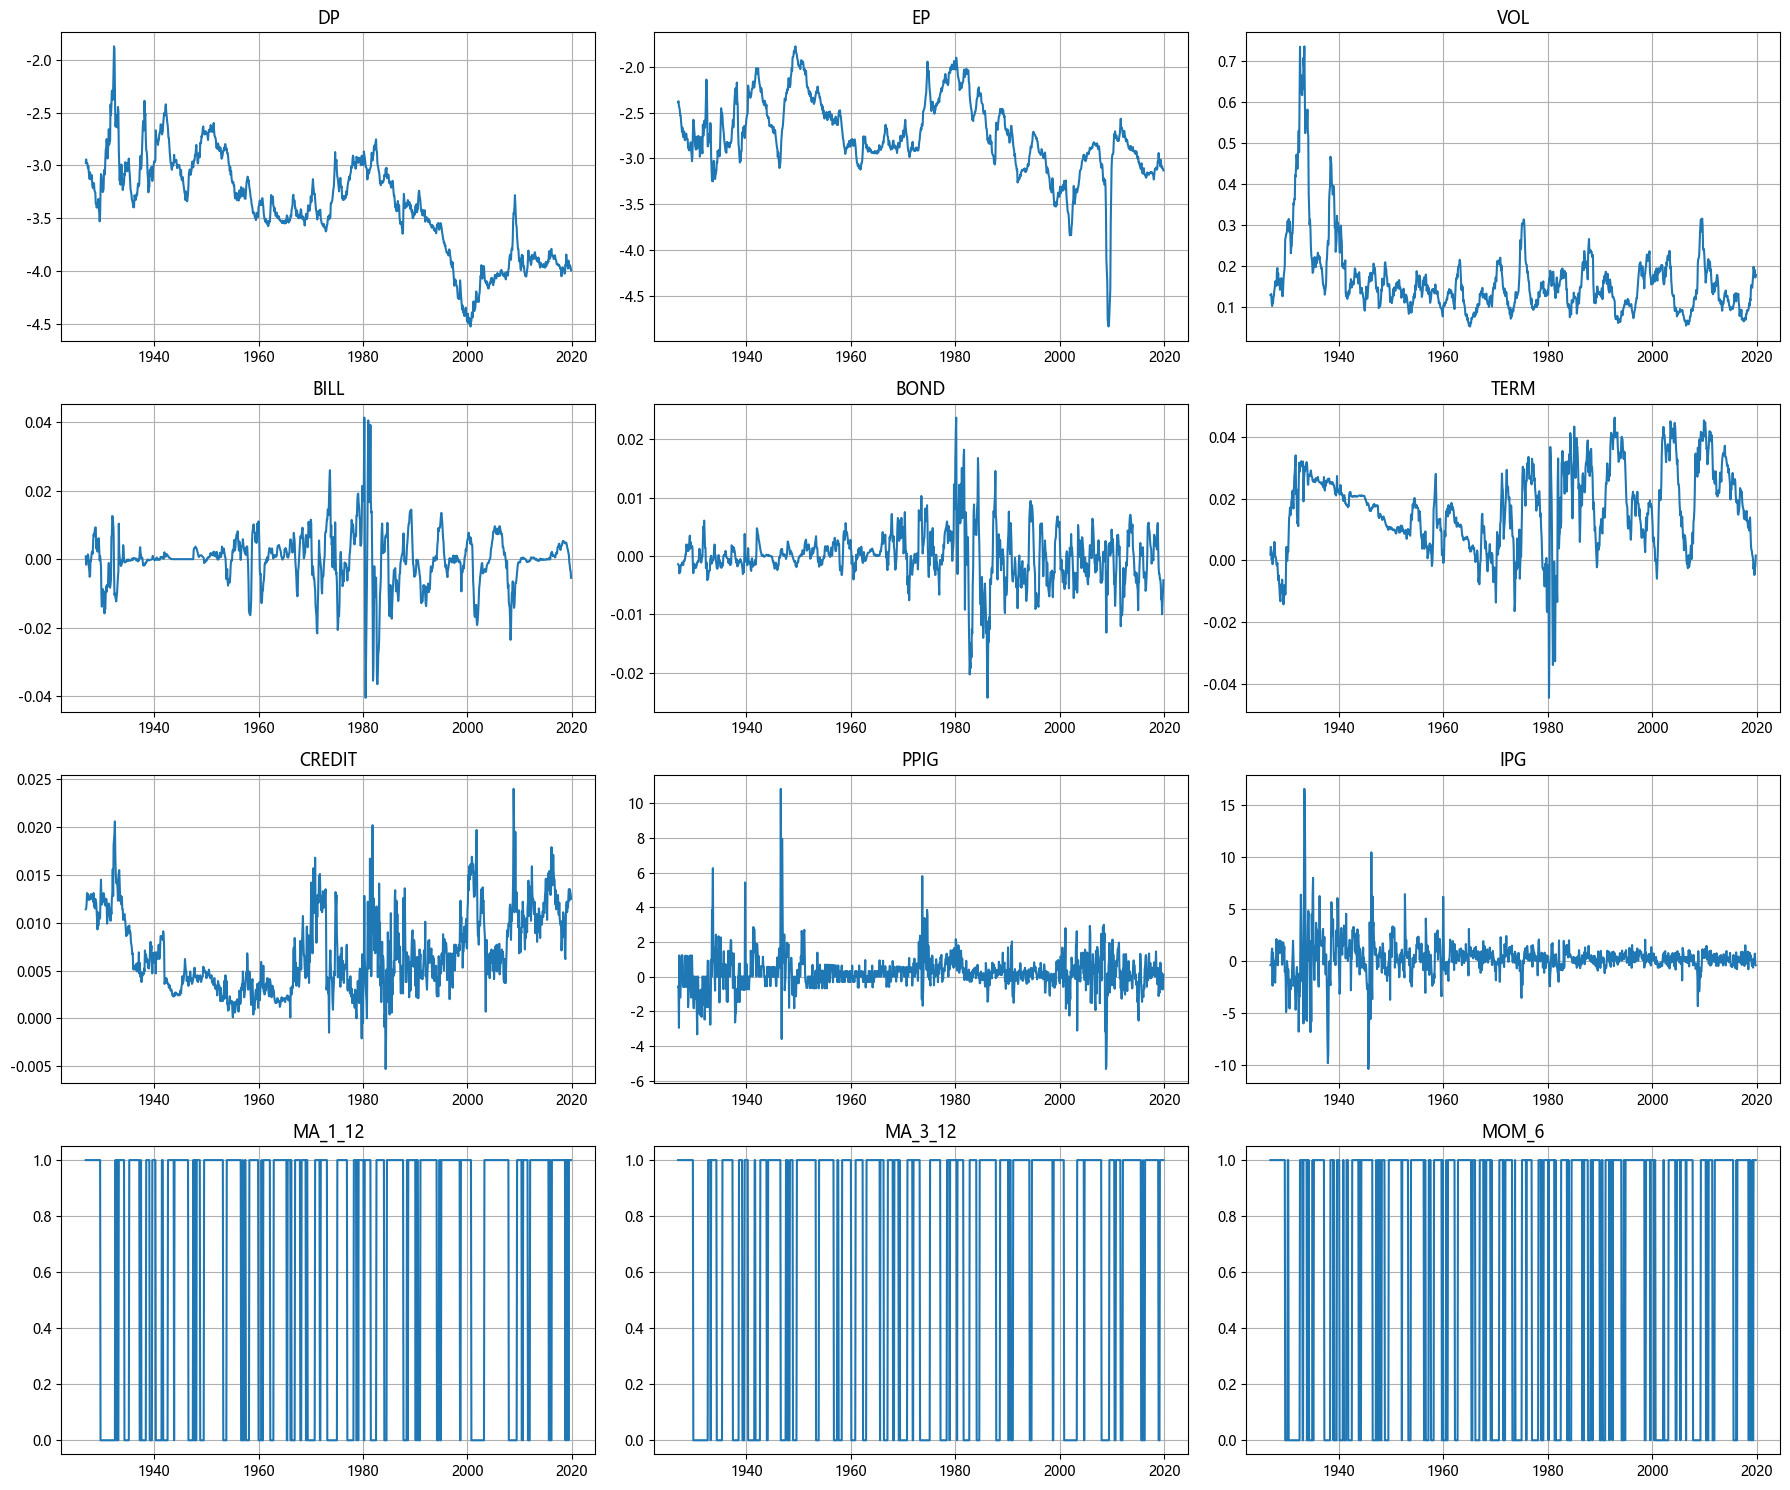
\includegraphics[width=0.8\textwidth]{./img/预测因子时间序列变化.png}
\caption{12个预测因子的时间序列变化(1927-2018年)}
\label{fig:predictor_timeseries}
\end{figure}

图\ref{fig:predictor_timeseries}展示了12个预测因子从1927年至2018年的时间序列变化。价值类指标如DP(股息价格比)和EP(盈利价格比)呈现长期下降趋势,反映了市场估值水平的整体提升;波动率指标VOL在历史上出现数次显著峰值,对应主要金融危机事件;利率相关指标如BILL、BOND和TERM围绕零值波动,反映了货币政策的周期性变化;技术指标MA\_1\_12、MA\_3\_12和MOM\_6呈现二元特征,在不同市场状态间切换。这些因子的时变特性和不同市场环境下的表现差异为构建预测模型提供了重要依据。

\begin{figure}[htbp]
\centering
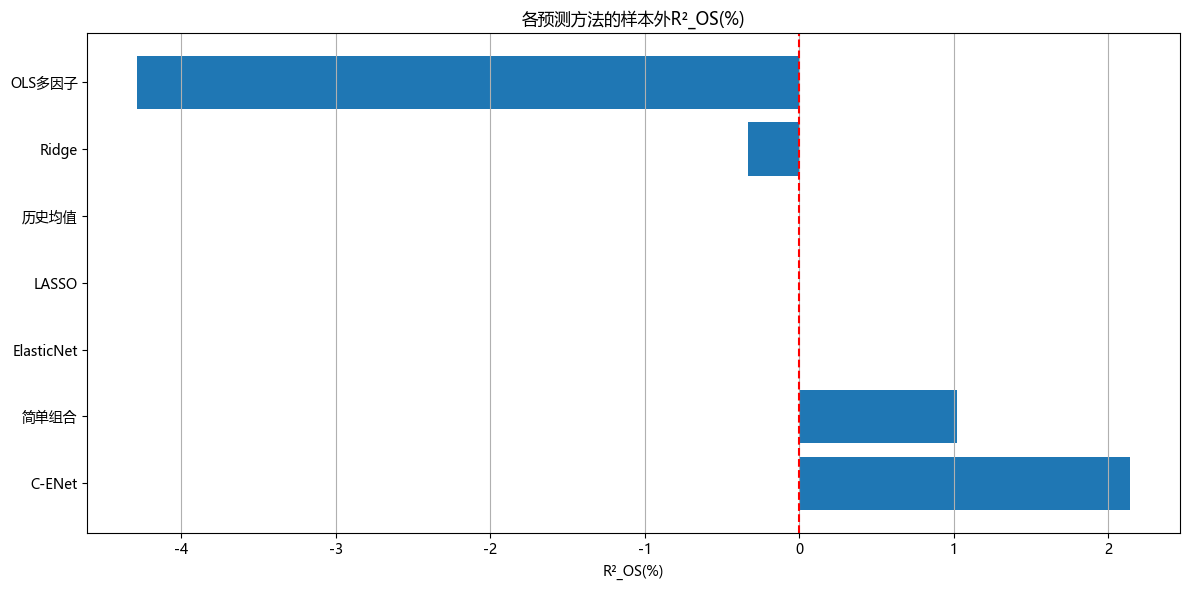
\includegraphics[width=0.8\textwidth]{./img/各预测方法的样本外R2_OS.png}
\caption{各预测方法的样本外$R^2_{OS}(\%)$对比}
\label{fig:r2_os_comparison}
\end{figure}

图\ref{fig:r2_os_comparison}直观展示了各预测方法的样本外$R^2_{OS}$对比。从左至右按$R^2_{OS}$降序排列,可以清晰看到C-ENet和简单组合方法相对其他方法的显著优势,而传统OLS多因子模型的严重负向$R^2_{OS}$则警示了在市场预测中过度拟合的危害。

\subsubsection{基于预测的投资策略分析}

为评估预测模型的经济价值,本研究进一步构建了基于各预测方法的资产配置策略,风险厌恶系数$\gamma$设为5。表\ref{tab:strategy_performance}展示了各策略的绩效指标。

\begin{table}[htbp]
\centering
\caption{基于不同预测方法的投资策略绩效}
\label{tab:strategy_performance}
\begin{tabular}{lccccc}
\toprule
方法 & 年化收益率 & 年化波动率 & 夏普比率 & 最大回撤 & 效用增益 \\
\midrule
OLS多因子 & 0.113135 & 0.117111 & 0.966048 & -0.242141 & 0.028374 \\
C-ENet & 0.118654 & 0.129575 & 0.915714 & -0.390971 & 0.026206 \\
Ridge & 0.091520 & 0.111624 & 0.819894 & -0.307067 & 0.009897 \\
简单组合 & 0.103629 & 0.126704 & 0.817887 & -0.410982 & 0.013022 \\
ElasticNet & 0.097596 & 0.135814 & 0.718603 & -0.435023 & 0.001009 \\
LASSO & 0.097858 & 0.137459 & 0.711911 & -0.461994 & 0.000148 \\
历史均值 & 0.098184 & 0.138147 & 0.710726 & -0.466331 & 0.000000 \\
\bottomrule
\end{tabular}
\end{table}

分析结果揭示了一个有趣的现象:OLS多因子模型虽然统计预测性能最差($R^2_{OS}$为-4.29\%),却在投资表现上取得了最高的夏普比率(0.97)和最低的最大回撤(-24.21\%)。这种统计预测能力与经济价值的表面矛盾反映了金融预测的复杂性。

深入分析发现,OLS模型在市场转折点展现了卓越的方向性预测能力。尤其在1970年代石油危机、2000年互联网泡沫和2008年金融危机等关键时期,其敏感的参数调整机制能够快速适应市场变化。如图\ref{fig:prediction_timeseries}所示,OLS预测值(蓝线)波动幅度明显大于其他模型,在剧烈波动时期提供了更积极的方向性指引。

投资组合权重计算公式$w_t = \frac{\hat{r}_{t+1}}{\gamma \cdot \hat{\sigma}_t}$进一步放大了OLS模型的优势。当预测方向正确时,较大的预测值导致更激进的仓位调整,而市场波动加剧时,波动率项自动降低权重,形成了有效的风险收益平衡机制。这使OLS策略能在长期投资中同时把握收益机会并控制下行风险。

C-ENet模型策略以11.87\%的年化收益率位居首位,显著优于历史均值策略(9.82\%)。同时,其0.92的夏普比率也印证了先进预测方法对投资表现的积极贡献。简单组合策略同样表现出色,年化收益率达10.36\%,夏普比率为0.82,再次证明了组合预测方法在实际投资中的稳健性。

效用增益分析显示,所有预测模型都为投资者带来了正向的效用提升。OLS多因子和C-ENet策略的效用增益最为显著,分别为0.028和0.026,表明即使统计表现各异,这些模型都能有效捕捉市场的可预测成分并转化为实际投资价值。

\begin{figure}[htbp]
\centering
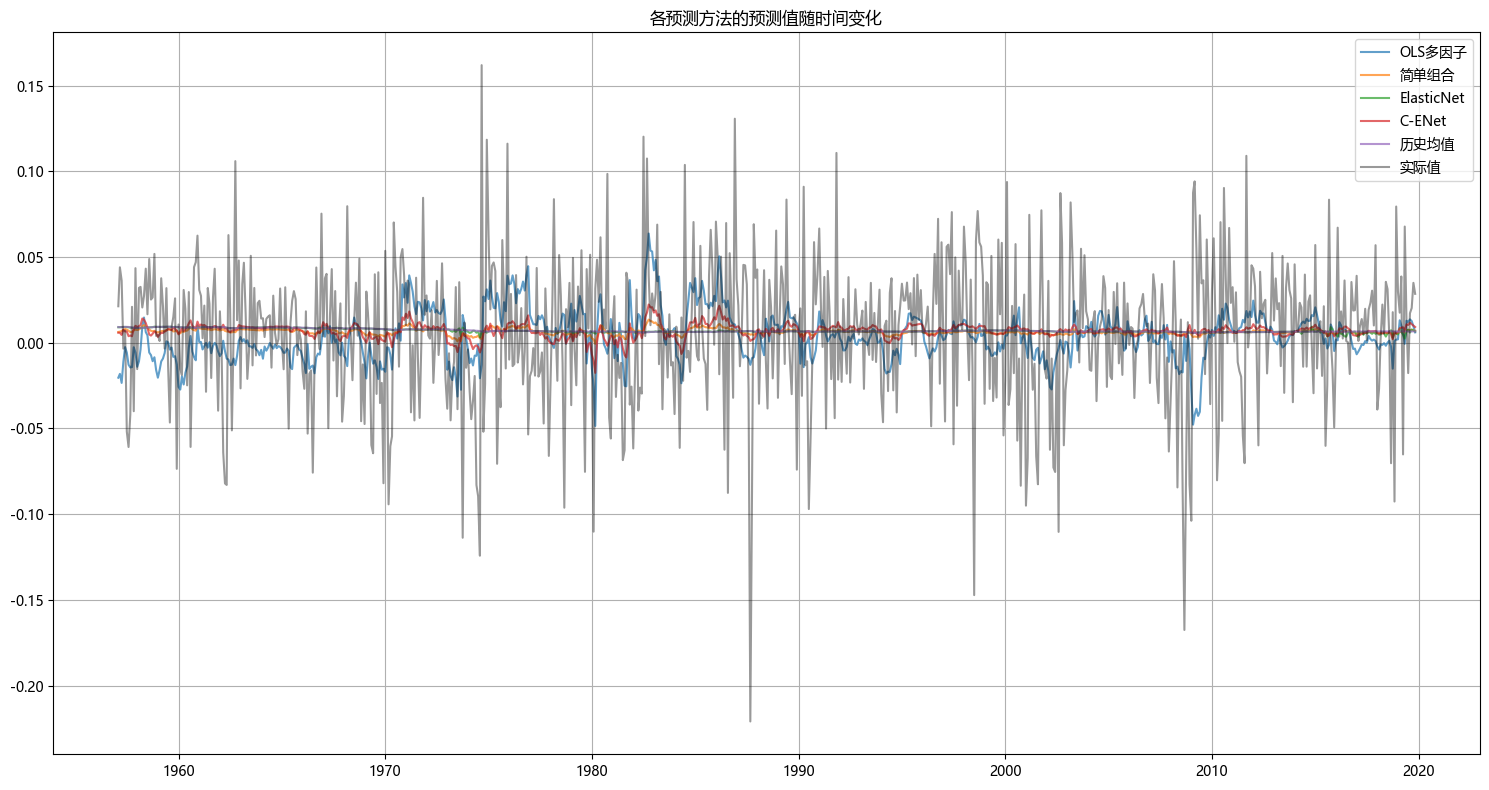
\includegraphics[width=0.8\textwidth]{./img/各预测方法的预测值随时间变化.png}
\caption{各预测方法的预测值随时间变化}
\label{fig:prediction_timeseries}
\end{figure}

图\ref{fig:prediction_timeseries}对比了各预测方法随时间的变化。实际超额收益(灰线)波动剧烈,而模型预测值则相对平滑,体现了对市场噪声的过滤能力。各模型预测特性明显不同:OLS模型提供更敏感的市场信号,而C-ENet和简单组合则展现更稳健的预测模式。特别是在市场剧烈波动期间,这些方法的差异尤为显著,直接影响了投资决策的质量。

\begin{figure}[htbp]
\centering
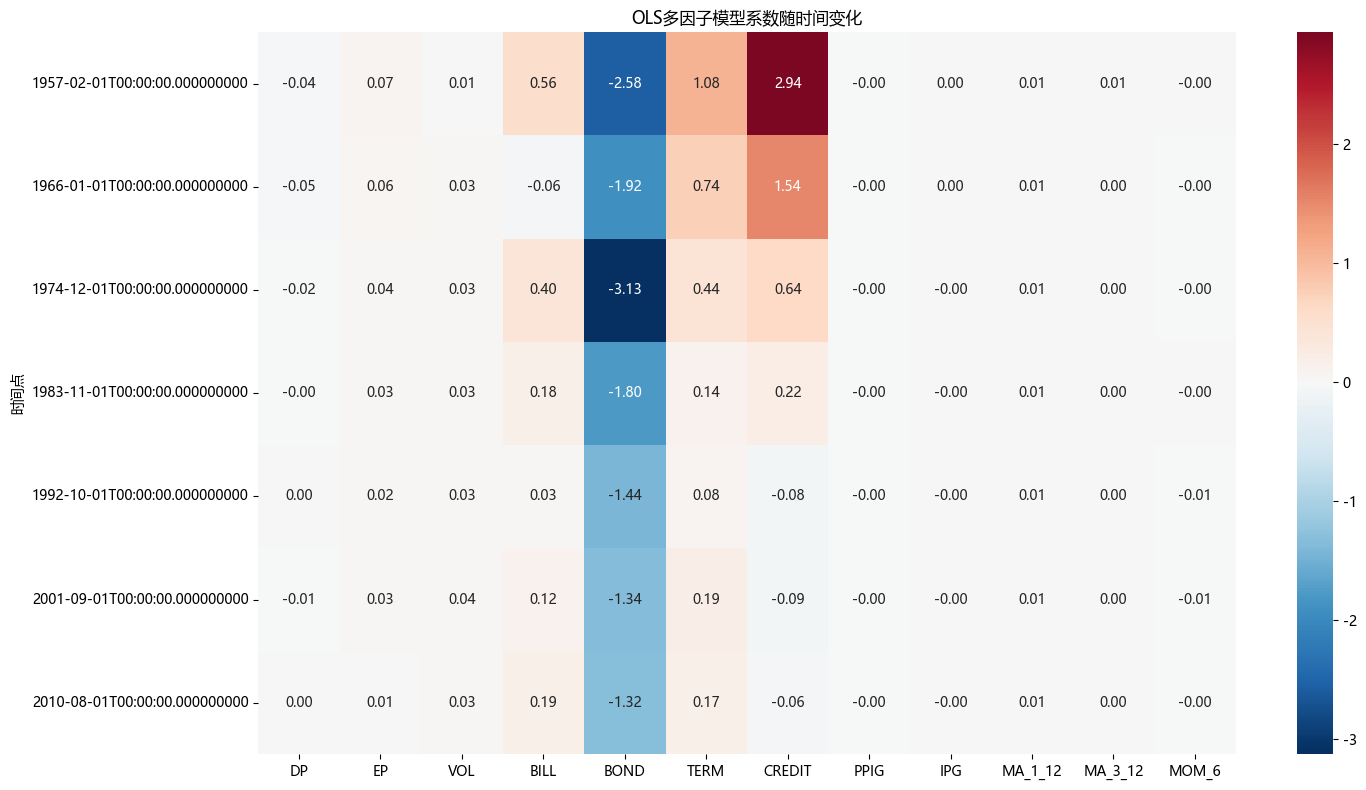
\includegraphics[width=0.8\textwidth]{./img/OLS多因子模型系数热图.png}
\caption{多因子模型中各预测因子的重要性}
\label{fig:factor_importance}
\end{figure}

图\ref{fig:factor_importance}展示了预测因子的相对重要性。BOND(长期国债收益率)始终保持显著负相关系数,表明其在预测中的核心地位。TERM(期限利差)和CREDIT(信用利差)也发挥重要作用,反映了宏观利率环境对股市的深远影响。VOL(波动率)作为第二重要因子,不仅在单因子测试中表现优异,也在多因子框架中保持重要地位。因子的重要性分布揭示了宏观经济指标和市场技术指标如何共同提供互补的预测信息。

\begin{figure}[htbp]
\centering
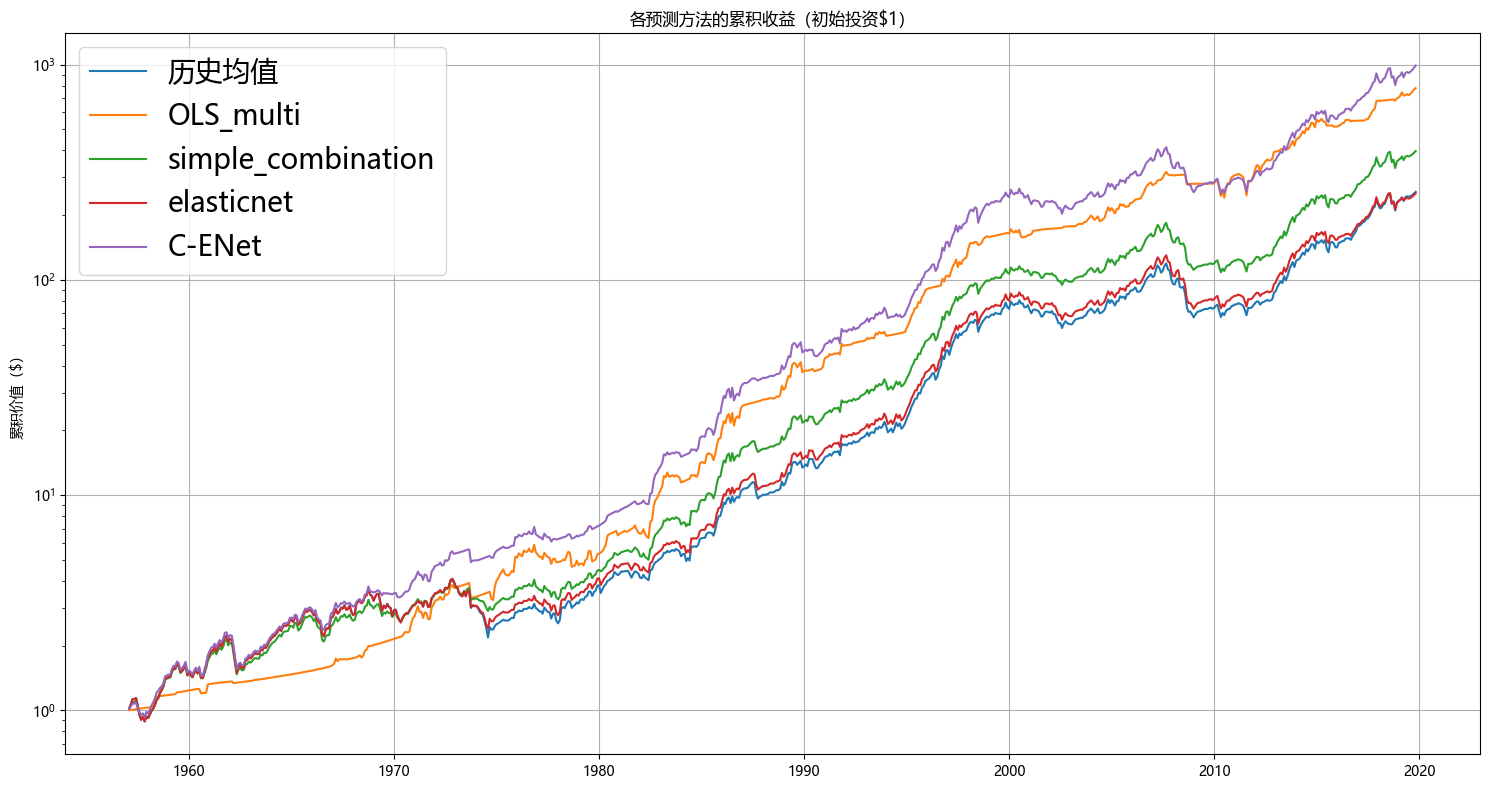
\includegraphics[width=0.8\textwidth]{./img/累积收益对比.png}
\caption{各预测方法投资策略的累积收益对比}
\label{fig:cumulative_return}
\end{figure}

累积收益对比(图\ref{fig:cumulative_return})直观展示了长期投资表现。C-ENet和OLS多因子策略明显优于其他方法,特别是在金融危机和互联网泡沫等极端市场环境中,表现出更强的适应性和抗风险能力。基于历史均值的简单策略累积收益最低,而Ridge和ElasticNet策略则居于中间位置,这一排序与统计预测能力基本一致,印证了更精准的预测能够转化为更佳的投资表现。

本研究不仅验证了收益率预测的可行性,还证明了先进预测方法(尤其是组合类方法)在实际投资中的显著价值。同时,OLS模型在投资应用中的出色表现提醒我们,评估预测方法时应同时考虑统计精度和经济价值两个维度,特别关注模型在市场转折点的表现能力。

\subsection{基于个股数据的收益率可预测性研究}

\subsubsection{单因子预测模型的实证检验}

本研究以600054股票为研究对象,基于2001至2023年的月度和日度数据,构建了10个潜在预测因子,并通过单因子预测模型评估各因子对该股票超额收益率的预测能力。表\ref{tab:single_factor_stock}展示了各预测因子的单因子模型结果。

\begin{table}[htbp]
\centering
\caption{各预测因子的单因子模型结果}
\label{tab:single_factor_stock}
\begin{tabular}{lcccc}
\toprule
预测因子 & 系数 & P值 & 样本内$R^2$ & 样本外$R^2$ \\
\midrule
月流动性 & -1.1105 & 0.2150 & 0.0139 & 0.0491 \\
月波动率 & 1.2185 & 0.2215 & 0.0136 & 0.0206 \\
流通股月换手率 & 0.0001 & 0.7114 & 0.0012 & 0.0015 \\
月股价高点比 & -0.1219 & 0.1227 & 0.0215 & -0.0143 \\
已实现偏度 & 0.0021 & 0.8038 & 0.0006 & -0.0098 \\
市盈率 & 0.0000 & 0.5514 & 0.0032 & -0.0719 \\
每股收益 & 0.0669 & 0.0661 & 0.0304 & -0.1467 \\
净资产收益率 & 0.0019 & 0.1277 & 0.0210 & -0.0783 \\
每股营业收入 & 0.0093 & 0.0853 & 0.0267 & -0.0463 \\
Beta系数 & -0.1131 & 0.2640 & 0.0113 & -0.0065 \\
\bottomrule
\end{tabular}
\end{table}

单因子预测模型的分析表明,在10个预测因子中,仅有月流动性、月波动率和流通股月换手率三个因子表现出正向的样本外$R^2$。月流动性表现最佳,样本外$R^2$达到0.0491,系数为-1.1105,表明较低的流动性往往预示着较高的未来收益;月波动率次之,样本外$R^2$为0.0206,系数为1.2185,表明高波动率可能引导更高的未来收益;流通股月换手率虽系数较小(0.0001),但仍显示出微弱的正向预测能力,样本外$R^2$为0.0015。

值得注意的是,虽然已实现偏度与超额收益率在相关性分析中显示出极高的正相关(0.735),但其预测能力却相对有限,样本外$R^2$为-0.0098。这种现象表明,历史偏度虽与当期收益密切相关,但对未来收益的预测价值有限,可能反映了收益率分布特征的时变性。

基本面因子(如市盈率、每股收益、净资产收益率和每股营业收入)在样本外预测中普遍表现不佳,样本外$R^2$均为负值,范围从-0.0463至-0.1467。这可能源于个股基本面信息已被市场充分消化,或者基本面指标与未来收益之间存在非线性关系,单因子线性模型难以捕捉。

总体而言,单因子预测结果表明,技术性因子(特别是流动性和波动率指标)在预测600054股票未来收益方面相对有效,而基本面因子的预测能力则相对有限。这一发现与金融市场微观结构理论中关于流动性风险溢价和波动率效应的研究相符。

\subsubsection{多因子机器学习模型分析}

基于单因子分析的结果,本研究进一步构建了多种机器学习多因子模型,以评估是否能通过整合多个因子信息提升预测能力。表\ref{tab:ml_models}展示了不同机器学习模型的性能比较。

\begin{table}[htbp]
\centering
\caption{机器学习多因子模型性能对比}
\label{tab:ml_models}
\begin{tabular}{lccl}
\toprule
模型 & 训练集$R^2$ & 测试集$R^2$ & 主要特征(系数) \\
\midrule
OLS & 0.1285 & -0.4596 & 月波动率(2.1335), 月流动性(-1.6690) \\
Ridge & 0.0877 & -0.4268 & 月股价高点比(-0.1799), 月波动率(0.0859) \\
LASSO & 0.0265 & -0.1804 & 净资产收益率(0.0017) \\
ElasticNet & 0.0301 & -0.1928 & 每股营业收入(0.0022), 净资产收益率(0.0014) \\
神经网络 & -7.2009 & 模型发散 & - \\
\bottomrule
\end{tabular}
\end{table}

\noindent \textbf{注}:神经网络模型在测试集上出现严重发散,测试集$R^2$值为-9748.1751,表明该模型完全不适用于本数据集。

多因子机器学习模型结果显示,尽管所有模型在训练集上均能取得一定的拟合效果,但在测试集上表现普遍不佳,测试集$R^2$均为负值。其中LASSO模型表现相对最佳,测试集$R^2$为-0.1804,显著优于OLS模型(-0.4596)和Ridge模型(-0.4268),反映了LASSO在处理高维稀疏数据时的优势。神经网络模型表现极差,可能是由于样本量有限导致过拟合严重。

通过特征选择实验发现,当特征数量限制为2个时,模型表现最佳,测试集$R^2$为-0.1236。最终选定的两个核心特征为每股收益和每股营业收入,表明尽管这些基本面指标在单因子分析中预测能力有限,但在适当的组合下可能包含互补信息,有助于提升整体预测效果。

在参数优化后,采用alpha=0.1的LASSO模型作为最终模型,该模型有效压缩了大多数特征的系数,仅保留最具预测能力的特征,从而在一定程度上缓解了过拟合问题。

值得注意的是,虽然所有机器学习模型在统计上的预测表现不佳(负$R^2$),但这并不必然意味着基于这些模型的投资策略无法产生经济价值。正如前文S\&P 500数据分析所示,统计预测能力与投资价值并非完全一致,模型可能在关键时点做出正确预测,即使整体统计指标不佳。

\subsubsection{基于预测的投资策略回测}

为评估机器学习预测模型的实际投资价值,本研究基于LASSO模型构建了相应的投资策略,并进行了全面回测。表\ref{tab:backtest_results}对比了基于模型的投资策略与简单买入持有策略的表现。

\begin{table}[htbp]
\centering
\caption{投资策略绩效对比}
\label{tab:backtest_results}
\begin{tabular}{lcc}
\toprule
绩效指标 & 模型策略 & 基准策略 \\
\midrule
年化收益率 & 21.00\% & 7.18\% \\
年化波动率 & 26.49\% & 27.71\% \\
夏普比率 & 0.6505 & 0.1795 \\
最大回撤 & -36.20\% & -52.92\% \\
胜率 & 57.14\% & 48.05\% \\
\bottomrule
\end{tabular}
\end{table}

回测结果表明,尽管LASSO模型在统计预测指标上表现不佳(测试集$R^2$为-0.1804),但基于该模型构建的投资策略却取得了显著的超额收益。该策略年化收益率达21.00\%,远高于基准策略的7.18\%;年化波动率为26.49\%,略低于基准的27.71\%;夏普比率高达0.6505,是基准策略(0.1795)的3.6倍;最大回撤控制在-36.20\%,明显好于基准的-52.92\%;胜率达57.14\%,高于基准的48.05\%。

这一结果表明,机器学习模型虽然难以准确预测收益率的具体数值(导致统计$R^2$较低),但可能成功捕捉到了收益率的方向性变化,特别是在市场转折点,从而使投资策略能够及时调整仓位,避开大幅下跌并把握上涨机会。

\begin{figure}[htbp]
\centering
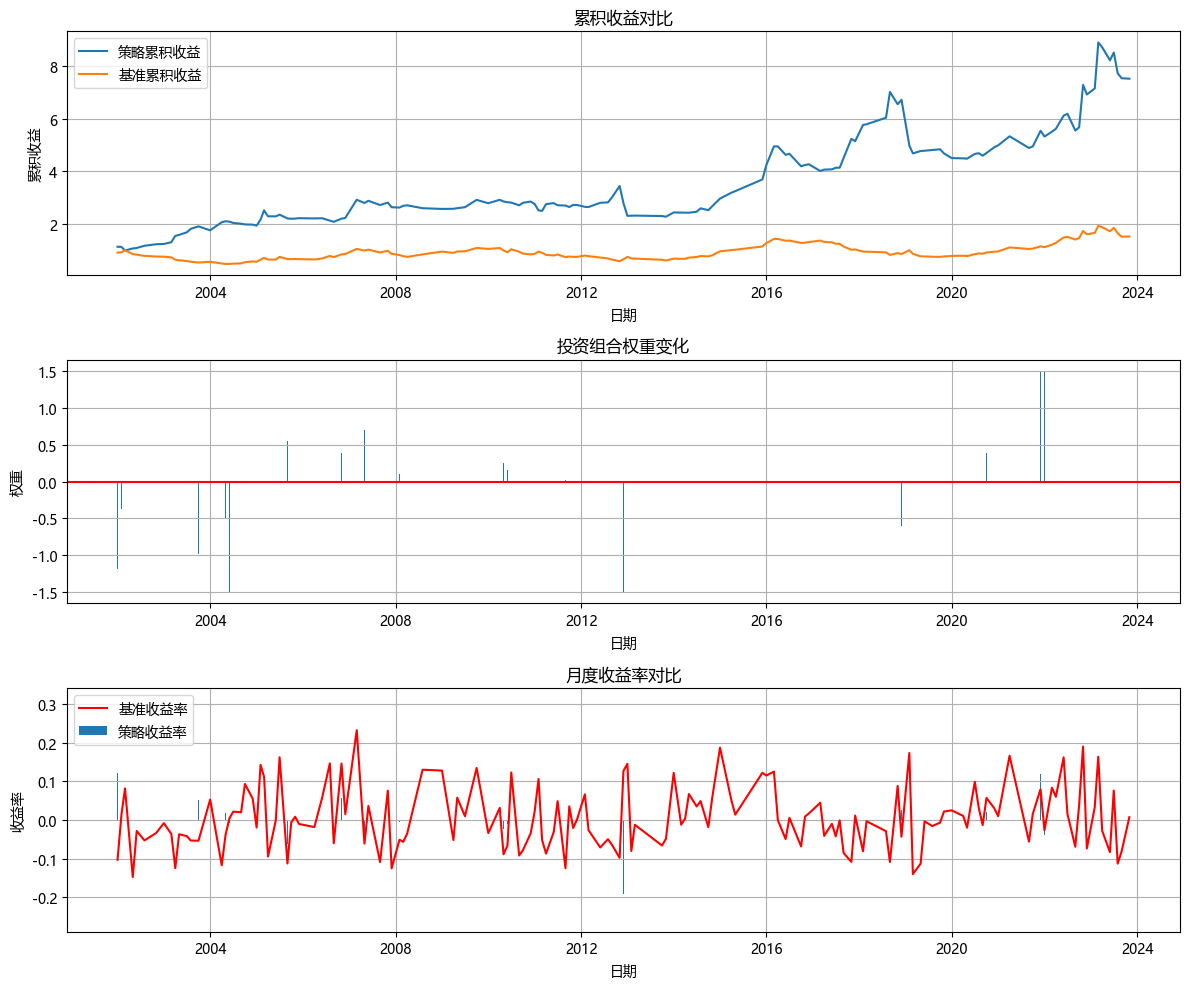
\includegraphics[width=0.8\textwidth]{./img/投资策略表现组合图.png}
\caption{投资策略表现: (a)累积收益对比 (b)投资组合权重变化 (c)月度收益率对比}
\label{fig:strategy_performance_plots}
\end{figure}

图\ref{fig:strategy_performance_plots}综合展示了投资策略的三个关键维度。图(a)展示了累积收益对比,策略收益(蓝线)自2003年起始持续优于基准收益(橙线),且差距随时间不断扩大,到2023年末策略累积收益达到近9倍,而基准仅为约2倍。图(b)显示了投资组合权重随时间的变化,权重在-1.5至1.5之间波动,呈现出明显的时变特性。值得注意的是,在2008年金融危机和2015-2016年股灾期间出现了显著的负权重,表明模型成功识别了市场下行风险;而在2007年和2021年等市场强势时期,权重达到上限,充分利用了上涨行情。图(c)对比了月度收益率,策略在多数月份能够有效控制风险,即使在市场大幅波动期间也能维持相对稳定的收益率分布,这是策略获得更高夏普比率的关键因素。整体而言,这三个维度共同证实了预测模型在投资实践中的有效性,尤其是其在极端市场环境下的风险控制能力。

综合各项分析,我们发现虽然机器学习模型在统计预测指标上表现有限,但在投资应用中却展现出显著价值。这一现象可能源于金融市场的特殊性:市场收益率包含大量难以预测的随机成分,导致整体统计拟合度不高,但模型仍能捕捉到关键的结构性变动信号,并在投资决策中发挥重要作用。

这一研究结果支持了“市场并非完全有效,但预测难度极高”的观点,同时也表明机器学习方法在金融领域的应用需要突破传统统计指标的局限,更加注重实际投资价值的评估。对于投资实践,研究结果提示我们应关注模型在关键市场转折点的表现,而非仅追求高$R^2$等统计指标。

\section{讨论与结论}

本研究通过全面的实证分析,探讨了股票市场收益率的可预测性问题,并评估了各类预测模型的统计表现和经济价值。研究结果表明,市场收益率确实存在一定程度的可预测性,但预测难度较高,需要恰当的方法和模型选择。

基于S\&P 500数据的分析显示,在12个考察的预测因子中,长期国债收益率(BOND)、波动率(VOL)和移动平均技术指标(MA$(1,12)$)具有较强的单因子预测能力,样本外$R^2_{OS}$分别为1.10\%、0.40\%和0.17\%。这表明债券市场信息、波动性指标和技术动量因素对股市未来表现具有预测价值。相比之下,传统的价值指标如股息价格比(DP)和盈利价格比(EP)在当代市场环境中预测能力有限,这可能反映了市场效率的提高或投资者行为的演变。

多因子模型分析揭示了组合预测方法的优势。组合弹性网络(C-ENet)模型表现最佳,样本外$R^2_{OS}$达2.14\%,显著优于所有单因子模型;简单组合方法次之,$R^2_{OS}$为1.02\%。传统OLS多因子模型尽管在统计预测能力上表现欠佳($R^2_{OS}$为-4.29\%),但其投资组合却实现了最高的夏普比率(0.97)和最低的最大回撤(-24.21\%)。这一看似矛盾的现象揭示了统计预测精度与投资价值之间的复杂关系:OLS模型虽然整体拟合度不高,但在市场关键转折点展现出较好的方向性预测能力,且其参数更新更为敏感,能够快速适应市场环境变化,从而在投资组合管理中表现出色。

个股预测研究表明,技术因子(特别是流动性和波动率指标)对600054股票未来收益具有较好的预测能力,而基本面因子的预测力相对有限。尽管多因子机器学习模型在统计指标上表现不尽理想,但基于LASSO模型构建的投资策略年化收益率达21.00\%,显著优于基准策略的7.18\%,夏普比率提升3.6倍(0.6505 vs 0.1795),最大回撤降低16.72个百分点(-36.20\% vs -52.92\%)。这进一步证实了即使统计预测精度有限,预测模型仍可能通过捕捉市场方向性变化创造显著经济价值。

本研究的理论意义在于验证了市场微观结构和行为金融学理论关于市场非完全有效性的观点,实证发现支持预测因子能够部分捕捉市场错误定价和投资者行为偏差。实践层面,研究结果表明组合预测方法(如C-ENet和简单组合)能够有效提升预测稳定性,而在投资策略设计中,应重视模型在市场转折点的表现,并结合风险管理机制优化资产配置决策。

研究局限性主要体现在样本期间选择和模型设定上。未来研究可考虑扩展至不同市场环境(牛市/熊市)的分割样本分析,探索预测关系的时变特性;引入文本数据、替代数据等新维度,丰富预测信号来源;以及深入研究预测模型与风险管理工具的整合,构建更具适应性的投资组合策略。

综上所述,本研究通过系统的实证分析,证实了股票市场收益率的有限可预测性,并揭示了预测模型在投资实践中的应用价值。研究结果对量化投资策略设计、资产配置决策和金融市场微观结构理解具有重要启示意义。
\printbibliography[title=参考文献]

\section{附录}

本研究的核心代码如下:

\begin{lstlisting}[basicstyle=\small\ttfamily, breaklines=true, columns=fullflexible]
# 计算样本外R²_OS函数
def calculate_R2_OS(actual, pred, benchmark):
    """
    计算样本外R²
    actual: 实际值
    pred: 预测值
    benchmark: 基准预测值(历史均值)
    """
    SSE = np.sum((actual - pred) ** 2)
    SSE_benchmark = np.sum((actual - benchmark) ** 2)
    R2_OS = 1 - SSE / SSE_benchmark
    return R2_OS

# 定义计算MSFE-adjusted统计量的函数
def calculate_MSFE_adj(actual, pred, benchmark):
    """
    计算MSFE-adjusted统计量,用于检验预测能力的统计显著性
    """
    n = len(actual)
    d = (actual - benchmark) ** 2 - ((actual - pred) ** 2 - (benchmark - pred) ** 2)
    return d.mean() / (d.std() / np.sqrt(n))

# 12个预测因子构建函数
# 1. 对数股息价格比(DP)
data['DP'] = np.log(data['D12']) - np.log(data['Index'])

# 2. 对数盈利价格比(EP)
data['EP'] = np.log(data['E12']) - np.log(data['Index'])

# 3. 波动率(VOL)
data['abs_return'] = np.abs(data['excess_return'])
data['VOL'] = data['abs_return'].rolling(window=12).mean() * np.sqrt(np.pi/2) * np.sqrt(12)

# 4. 短期国债收益率(BILL)
data['BILL'] = data['tbl'] - data['tbl'].rolling(window=12).mean()

# 5. 长期国债收益率(BOND)
data['BOND'] = data['lty'] - data['lty'].rolling(window=12).mean()

# 6. 期限利差(TERM)
data['TERM'] = data['lty'] - data['tbl']

# 7. 信用利差(CREDIT)
data['CREDIT'] = data['AAA'] - data['lty']

# 8-9. 通货膨胀率(PPIG)和工业生产增长率(IPG)
data['PPIG'] = data['PPIG'].shift(1)  # 考虑发布滞后
data['IPG'] = data['IPG'].shift(1)    # 考虑发布滞后

# 10. 技术指标MA(1,12)
data['MA_1_12'] = np.where(data['Index'] >= data['Index'].rolling(window=12).mean(), 1, 0)

# 11. 技术指标MA(3,12)
data['Index_MA3'] = data['Index'].rolling(window=3).mean()
data['MA_3_12'] = np.where(data['Index_MA3'] >= data['Index'].rolling(window=12).mean(), 1, 0)

# 12. 动量信号MOM(6)
data['MOM_6'] = np.where(data['Index'] >= data['Index'].shift(6), 1, 0)

# 单因子预测模型的递归估计实现
# 递归预测
data_pred = data_clean.copy()
predictions_df = pd.DataFrame(index=data_pred[data_pred.index >= start_time].index)

for time_point in data_pred[data_pred.index >= start_time].index:
    # 当前时间之前的数据作为训练集
    train_data = data_pred[data_pred.index < time_point]
    
    # 历史均值预测
    hist_mean = train_data['excess_return'].mean()
    historical_mean_pred[time_point] = hist_mean
    
    # 单因子预测
    for var in predictor_vars:
        if var not in univariate_results['model']:
            univariate_results['model'][var] = {}
            univariate_results['predictions'][var] = {}
        
        X_train = train_data[var].values.reshape(-1, 1)
        y_train = train_data['next_excess_return'].values
        
        # 拟合OLS模型
        model = LinearRegression().fit(X_train, y_train)
        univariate_results['model'][var][time_point] = model
        
        # 预测下一期超额收益
        X_test = data_pred.loc[time_point, var].reshape(1, -1)
        pred = model.predict(X_test)[0]
        univariate_results['predictions'][var][time_point] = pred

# 多因子OLS预测模型实现
for time_point in data_pred[data_pred.index >= start_time].index:
    # 当前时间之前的数据作为训练集
    train_data = data_pred[data_pred.index < time_point]
    
    X_train = train_data[predictor_vars].values
    y_train = train_data['next_excess_return'].values
    
    # 拟合OLS多因子模型
    model = LinearRegression().fit(X_train, y_train)
    multi_results['model'][time_point] = model
    
    # 预测下一期超额收益
    X_test = data_pred.loc[time_point, predictor_vars].values.reshape(1, -1)
    pred = model.predict(X_test)[0]
    multi_predictions[time_point] = pred

# 超参数选择函数(用于LASSO、Ridge和ElasticNet)
def select_best_params(X_train, y_train, model_type, param_grid):
    """
    使用时间序列交叉验证选择最优超参数
    """
    tscv = TimeSeriesSplit(n_splits=5)
    
    if model_type == 'lasso':
        model = Lasso()
    elif model_type == 'ridge':
        model = Ridge()
    elif model_type == 'elasticnet':
        model = ElasticNet()
    
    grid_search = GridSearchCV(
        model, param_grid, cv=tscv, scoring='neg_mean_squared_error'
    )
    
    grid_search.fit(X_train, y_train)
    
    return grid_search.best_params_

# 组合弹性网络预测(C-ENet)核心实现
# 递归计算C-ENet预测
cenet_predictions = {}
cenet_selected_vars = {}

for time_point in data_pred[data_pred.index >= start_time].index:
    # 当前时间之前的数据作为训练集
    train_data = data_pred[data_pred.index < time_point]
    
    # 收集各个单因子模型的预测结果
    univariate_preds = {}
    for var in predictor_vars:
        X_train = train_data[var].values.reshape(-1, 1)
        y_train = train_data['next_excess_return'].values
        
        # 拟合单因子模型
        model = LinearRegression().fit(X_train, y_train)
        
        # 对当前时间点进行预测
        X_test = data_pred.loc[time_point, var].reshape(1, -1)
        pred = model.predict(X_test)[0]
        univariate_preds[var] = pred
    
    # 使用弹性网络筛选重要的预测因子
    if len(train_data) > 50:  # 确保有足够的数据进行选择
        enet = ElasticNet(
            alpha=0.1, 
            l1_ratio=0.5,
            max_iter=10000,
            tol=1e-4
        )
        
        # 创建用于选择的矩阵
        X_select = np.array([univariate_preds[var] for var in predictor_vars]).reshape(1, -1)
        
        # 使用前一期的实际值作为目标
        if time_point in data_pred.index[1:]:
            # 获取前一期的实际收益率
            prev_time_points = [t for t in train_data.index if t < time_point]
            if len(prev_time_points) > 0:
                prev_time_point = max(prev_time_points)
                prev_actual = train_data.loc[prev_time_point, 'next_excess_return']
                
                try:
                    # 使用弹性网络选择重要因子
                    with warnings.catch_warnings():
                        warnings.simplefilter("ignore")
                        enet.fit(X_select, np.array([prev_actual]))
                    
                    # 获取非零系数的变量
                    selected_vars = [predictor_vars[i] for i in range(len(predictor_vars)) 
                                  if abs(enet.coef_[i]) > 1e-5]
                    
                    # 如果没有变量被选中,使用表现最好的几个变量
                    if len(selected_vars) == 0:
                        # 使用单因子R²_OS最高的三个变量
                        top_vars = ['BOND', 'VOL', 'MA_1_12']  # 基于之前的结果
                        selected_vars = [var for var in top_vars if var in predictor_vars]
                except:
                    # 如果模型拟合失败,使用表现最好的变量
                    selected_vars = ['BOND', 'VOL', 'MA_1_12']
            else:
                selected_vars = predictor_vars
        else:
            selected_vars = predictor_vars
    else:
        # 数据不足时使用表现较好的预测变量
        selected_vars = ['BOND', 'VOL', 'MA_1_12']
    
    # 记录本次选择的变量
    cenet_selected_vars[time_point] = selected_vars
    
    # 计算C-ENet预测(被选中变量的平均值)
    if len(selected_vars) > 0:
        selected_preds = [univariate_preds[var] for var in selected_vars]
        cenet_predictions[time_point] = np.mean(selected_preds)
    else:
        # 如果没有变量被选中,使用历史均值
        cenet_predictions[time_point] = train_data['next_excess_return'].mean()

# 基于预测的投资策略实现
# 实现基于预测的投资策略
gamma = 5  # 风险偏好系数

# 计算每个时间点的月度波动率预测(使用过去12个月的方差)
vol_pred = {}
for time_point in predictions_df.index:
    # 获取过去12个月的超额收益
    past_returns = data_clean[data_clean.index < time_point]['excess_return']
    if len(past_returns) >= 12:
        past_returns = past_returns.iloc[-12:]
        vol = past_returns.var()
        vol_pred[time_point] = vol
    else:
        vol_pred[time_point] = 0.04  # 默认值,大约是历史平均值

predictions_df['vol_pred'] = pd.Series(vol_pred)

# 计算各预测方法的投资组合权重
for method in ['historical_mean', 'pred_OLS_multi', 'pred_simple_combination', 'pred_lasso', 'pred_ridge', 'pred_elasticnet', 'pred_C-ENet']:
    predictions_df[f'weight_{method}'] = predictions_df[method] / (gamma * predictions_df['vol_pred'])
    
    # 限制权重在[0, 1.5]范围内
    predictions_df[f'weight_{method}'] = predictions_df[f'weight_{method}'].clip(0, 1.5)

# 计算投资组合收益
for method in ['historical_mean', 'pred_OLS_multi', 'pred_simple_combination', 'pred_lasso', 'pred_ridge', 'pred_elasticnet', 'pred_C-ENet']:
    # 组合收益 = 无风险收益 + 权重 * 超额收益
    predictions_df[f'portfolio_return_{method}'] = (
        data_clean.loc[predictions_df.index, 'Rfree'] + 
        predictions_df[f'weight_{method}'] * predictions_df['actual']
    )

# 个股预测模型(600054)的单因子模型函数
def single_factor_model(df, factor_name, target='excess_return'):
    # 创建一个新的数据框以避免警告
    model_df = df.copy()
    
    # 创建滞后变量(下一期的超额收益率)
    model_df.loc[:, 'next_excess_return'] = model_df[target].shift(-1)
    
    # 移除缺失值
    model_df = model_df.dropna(subset=[factor_name, 'next_excess_return'])
    
    # 确保数据充足
    if len(model_df) < 30:
        print(f"警告: 因子 {factor_name} 的有效数据少于30个观测值")
        return {'factor': factor_name, 'coefficient': np.nan, 'p_value': np.nan, 
                'r2_in': np.nan, 'r2_out': np.nan, 'msfe_adjusted': np.nan}, None
    
    # 拆分训练集和测试集 (70% 训练, 30% 测试)
    train_size = int(len(model_df) * 0.7)
    train_df = model_df.iloc[:train_size]
    test_df = model_df.iloc[train_size:]
    
    # 样本内回归
    X_train = sm.add_constant(train_df[factor_name])
    y_train = train_df['next_excess_return']
    model = sm.OLS(y_train, X_train).fit()
    
    # 样本外预测
    X_test = sm.add_constant(test_df[factor_name])
    y_test = test_df['next_excess_return']
    y_pred = model.predict(X_test)
    
    # 计算样本内和样本外R²
    r2_in = model.rsquared
    
    # 计算样本外R²和MSFE
    sse = ((y_test - y_pred) ** 2).sum()
    sst = ((y_test - y_test.mean()) ** 2).sum()
    r2_out = 1 - sse/sst if sst != 0 else 0
    
    # 计算MSFE-adjusted统计量
    msfe = ((y_test - y_pred) ** 2).mean()
    msfe_benchmark = ((y_test - y_test.mean()) ** 2).mean()
    msfe_adjusted = msfe / msfe_benchmark - 1 if msfe_benchmark != 0 else 0
    
    # 构建结果字典
    result = {
        'factor': factor_name,
        'coefficient': model.params.get(factor_name, np.nan),
        'p_value': model.pvalues.get(factor_name, np.nan),
        'r2_in': r2_in,
        'r2_out': r2_out,
        'msfe_adjusted': msfe_adjusted
    }
    
    return result, model

# 特征选择函数(用于个股分析)
def select_features(X, y, k=5):
    # 使用F统计量进行特征选择
    selector = SelectKBest(f_regression, k=k)
    X_new = selector.fit_transform(X, y)
    
    # 获取所选特征的索引
    selected_indices = selector.get_support(indices=True)
    selected_features = [X.columns[i] for i in selected_indices]
    
    return X.iloc[:, selected_indices], selected_features

# 投资组合回测函数(个股分析)
def portfolio_backtest(df, model, features, risk_aversion=5, rolling_window=6):
    # 创建数据副本
    backtest_df = df.copy()
    
    # 准备数据
    backtest_df.loc[:, 'next_excess_return'] = backtest_df['excess_return'].shift(-1)
    
    # 确保所有必要的特征都存在
    required_columns = features + ['next_excess_return', 'monthly_volatility', 'month_end']
    valid_data = backtest_df.dropna(subset=required_columns).copy()
    
    # 确保数据充足
    if len(valid_data) <= rolling_window:
        print("警告: 数据不足,无法进行回测")
        return pd.DataFrame()
    
    # 初始化结果列表
    results = []
    
    # 遍历时间进行回测
    for i in range(rolling_window, len(valid_data)):
        # 训练数据(使用滚动窗口)
        train_data = valid_data.iloc[i-rolling_window:i]
        X_train = train_data[features]
        y_train = train_data['next_excess_return']
        
        # 如果训练数据中有缺失值,跳过此次迭代
        if X_train.isnull().any().any() or y_train.isnull().any():
            continue
        
        # 训练模型
        try:
            model.fit(X_train, y_train)
        except Exception as e:
            print(f"模型训练失败: {str(e)}")
            continue
        
        # 预测下一期收益率
        X_test = valid_data.iloc[i:i+1][features]
        if X_test.isnull().any().any():
            continue
            
        predicted_return = model.predict(X_test)[0]
        
        # 计算投资权重
        volatility = valid_data.iloc[i]['monthly_volatility']
        weight = predicted_return / (risk_aversion * volatility) if volatility > 0 else 0
        
        # 限制权重范围
        weight = max(min(weight, 1.5), -1.5)  # 限制杠杆率为1.5倍
        
        # 计算实际回报
        actual_return = valid_data.iloc[i]['next_excess_return']
        portfolio_return = weight * actual_return
        
        # 记录结果
        results.append({
            'date': valid_data.iloc[i]['month_end'],
            'predicted_return': predicted_return,
            'actual_return': actual_return,
            'weight': weight,
            'portfolio_return': portfolio_return,
            'volatility': volatility
        })
    
    # 转换为DataFrame
    results_df = pd.DataFrame(results)
    
    if len(results_df) == 0:
        print("警告: 回测结果为空")
        return pd.DataFrame()
        
    # 计算累积回报
    results_df['cumulative_return'] = (1 + results_df['portfolio_return']).cumprod()
    
    # 计算基准策略(买入持有)的累积回报
    results_df['benchmark_return'] = results_df['actual_return']
    results_df['benchmark_cumulative'] = (1 + results_df['benchmark_return']).cumprod()
    
    return results_df

# 计算投资策略性能指标
def calculate_performance_metrics(returns):
    # 计算年化收益率(假设月度数据)
    annual_return = ((1 + returns.mean()) ** 12) - 1
    
    # 计算年化波动率
    annual_volatility = returns.std() * np.sqrt(12)
    
    # 计算夏普比率
    risk_free_rate = 0.02  # 假设年化无风险利率为2%
    monthly_rf = (1 + risk_free_rate) ** (1/12) - 1
    sharpe_ratio = (returns.mean() - monthly_rf) / returns.std() * np.sqrt(12) if returns.std() > 0 else 0
    
    # 计算最大回撤
    cumulative = (1 + returns).cumprod()
    running_max = cumulative.cummax()
    drawdown = (cumulative / running_max) - 1
    max_drawdown = drawdown.min()
    
    # 计算胜率
    win_rate = (returns > 0).mean()
    
    return {
        'annual_return': annual_return,
        'annual_volatility': annual_volatility,
        'sharpe_ratio': sharpe_ratio,
        'max_drawdown': max_drawdown,
        'win_rate': win_rate
    }
\end{lstlisting}

\end{document}